\documentclass[lang=cn,newtx,10pt,scheme=chinese]{elegantbook}
\usepackage{realboxes}

\title{ESP32教程}
\author{左元}

\setcounter{tocdepth}{3}

\cover{cover.pdf}

% 本文档命令
\usepackage{array}
\newcommand{\ccr}[1]{\makecell{{\color{#1}\rule{1cm}{1cm}}}}

% 修改标题页的橙色带
\definecolor{customcolor}{RGB}{32,178,170}
\colorlet{coverlinecolor}{customcolor}
\usepackage{cprotect}

\newtcolorbox{marker}[1][]{enhanced,
  before skip=2mm,after skip=3mm,
  boxrule=0.4pt,left=5mm,right=2mm,top=1mm,bottom=1mm,
  colback=yellow!50,
  colframe=yellow!20!black,
  sharp corners,rounded corners=southeast,arc is angular,arc=3mm,
  underlay={%
    \path[fill=tcbcolback!80!black] ([yshift=3mm]interior.south east)--++(-0.4,-0.1)--++(0.1,-0.2);
    \path[draw=tcbcolframe,shorten <=-0.05mm,shorten >=-0.05mm] ([yshift=3mm]interior.south east)--++(-0.4,-0.1)--++(0.1,-0.2);
    \path[fill=yellow!50!black,draw=none] (interior.south west) rectangle node[white]{\Huge\bfseries !} ([xshift=4mm]interior.north west);
    },
  drop fuzzy shadow,#1}

\tcbuselibrary{listings, skins, breakable}
\usepackage[T1]{fontenc}
\usepackage[ttdefault=true]{AnonymousPro}
\definecolor{pblue}{rgb}{0.13,0.13,1}
\definecolor{pgreen}{rgb}{0,0.5,0}

\newtcblisting[auto counter, number within=chapter]{mycode}[1]{
    breakable,
    enhanced,
    attach boxed title to top right={yshift=-\tcboxedtitleheight},
    boxed title style={
        size=small,colback=gray!50,
        colframe=gray!50,
        sharp corners=downhill,
        arc=.5cm,
        top=1mm,bottom=1mm,left=1mm,right=1mm
    },
    fonttitle=\color{black}\itshape\ttfamily,
    colframe=gray!20,
    top=\tcboxedtitleheight,
    bottom=\tcboxedtitleheight,
    sharp corners=downhill,
    arc=.5cm,
    title={#1},
    listing only,
    listing options={
        escapechar=@,
        language=c,
        basicstyle=\fontfamily{AnonymousPro}\selectfont,
        keywordstyle=\bfseries\color{pblue},
        stringstyle=\bfseries\itshape\color{green!40!black},
        commentstyle=\bfseries\itshape\color{black!60},
        % Line numbers
        xleftmargin={0.75cm},
        numbers=left,
        stepnumber=1,
        firstnumber=1,
        numberfirstline=true,
        showspaces=false,
        showtabs=false,
        breaklines=true,
        showstringspaces=false,
        tabsize=1,
        emph={
            gpio_config_t, for, uint8_t, TextView, Toast, Button, EditText, ImageView, Typeface, Intent, WebView, WebSettings, SwipeRefreshLayout, RelativeLayout, Animation, AlertDialog, SharedPreferences, Editor, ToggleButton, CardView, LinearLayout, gradient, shape,
        },
        emphstyle={\bfseries\color{pblue}},
        frame=l
    }
}

\begin{document}

\maketitle
\frontmatter

\tableofcontents

\mainmatter

\chapter{ESP32简介}

ESP32-C3 SoC 芯片支持以下功能:

\begin{itemize}
  \item 2.4 GHz Wi-Fi
  \item 低功耗蓝牙
  \item 高性能 32 位 RISC-V 单核处理器
  \item 多种外设
  \item 内置安全硬件
\end{itemize}

ESP32-C3 采用 40 nm 工艺制成,具有最佳的功耗性能、射频性能、稳定性、通用性和可靠性,适用于各种应用场景和不同功耗需求。

此芯片由乐鑫公司开发。

\begin{marker}
  我们使用的芯片是 ESP32-C3 。
\end{marker}

\chapter{安装开发工具ESP-IDF}

ESP-IDF 需要安装一些必备工具,才能围绕 ESP32-C3 构建固件,包括 Python、Git、交叉编译器、CMake 和 Ninja 编译工具等。

在本入门指南中,我们通过 \textcolor{red}{命令行} 进行有关操作。

\begin{marker}
限定条件:

\begin{itemize}
\item 请注意 ESP-IDF 和 ESP-IDF 工具的安装路径不能超过 90 个字符,安装路径过长可能会导致构建失败。
\item Python 或 ESP-IDF 的安装路径中一定不能包含空格或括号。
\item 除非操作系统配置为支持 Unicode UTF-8,否则 Python 或 ESP-IDF 的安装路径中也不能包括特殊字符(非 ASCII 码字符)
\item 各种路径中不要有中文!
\end{itemize}

系统管理员可以通过如下方式将操作系统配置为支持 Unicode UTF-8:控制面板-更改日期、时间或数字格式-管理选项卡-更改系统地域-勾选选项 “Beta:使用 Unicode UTF-8 支持全球语言”-点击确定-重启电脑。
\end{marker}

\section{离线安装ESP-IDF}

点击\href{https://dl.espressif.com/dl/esp-idf/?idf=4.4}{链接}下载离线安装包。

\begin{figure}[!htb]
\centering

\includegraphics[width=0.9\textwidth]{1.png}
\caption{离线安装包}
\end{figure}

\section{安装内容}

安装程序会安装以下组件:

\begin{itemize}
\item 内置的 Python
\item 交叉编译器
\item OpenOCD
\item CMake 和 Ninja 编译工具
\item ESP-IDF
\end{itemize}

安装程序允许将程序下载到现有的ESP-IDF目录。

推荐将ESP-IDF下载到 \Colorbox{lightgrey}{\lstinline{%userprofile%\Desktop\esp-idf}}目录下,其中\Colorbox{lightgrey}{\lstinline}代表家目录。

\section{启动ESP-IDF环境}

安装结束时,如果勾选了 \Colorbox{lightgrey}{\lstinline{Run ESP-IDF PowerShell Environment}} 或 \Colorbox{lightgrey}{\lstinline{Run ESP-IDF Command Prompt (cmd.exe)}},安装程序会在选定的提示符窗口启动 ESP-IDF。

Run ESP-IDF PowerShell Environment:

\begin{figure}[!htb]
\centering
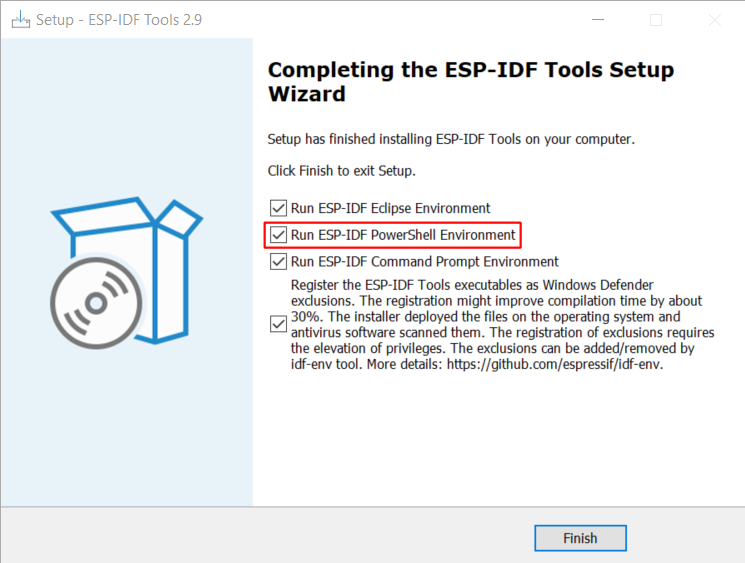
\includegraphics[width=0.9\textwidth]{esp-idf-installer-screenshot-powershell.png}
\caption{PowerShell}
\end{figure}

\chapter{创建工程}

现在,可以准备开发 ESP32 应用程序了。可以从 ESP-IDF 中 examples 目录下的 \Colorbox{lightgrey}{\lstinline{get-started/hello_world}} 工程开始。

\begin{marker}
    ESP-IDF 编译系统不支持 ESP-IDF 路径或其工程路径中带有空格。
\end{marker}

将 \Colorbox{lightgrey}{\lstinline{get-started/hello_world}} 工程复制至本地的 \Colorbox{lightgrey}{\lstinline{~/esp}} 目录下:

\begin{mycode}{复制工程命令}
$ cd %userprofile%\esp
$ xcopy /e /i %IDF_PATH%\examples\get-started\hello_world hello_world
\end{mycode}


\begin{marker}
    ESP-IDF 的 examples 目录下有一系列示例工程,可以按照上述方法复制并运行其中的任何示例,也可以直接编译示例,无需进行复制。
\end{marker}

\section{连接设备}

现在,请将 ESP32 开发板连接到 PC,并查看开发板使用的串口。

在 Windows 操作系统中,串口名称通常以 COM 开头。

\section{配置工程}

请进入 \Colorbox{lightgrey}{\lstinline{hello_world}} 目录,设置 ESP32-C3 为目标芯片,然后运行工程配置工具 menuconfig 。

\begin{mycode}{配置命令}
cd %userprofile%\esp\hello_world
idf.py set-target esp32c3
idf.py menuconfig
\end{mycode}

打开一个新工程后,应首先使用 \Colorbox{lightgrey}{\lstinline{idf.py set-target esp32c3}} 设置“目标”芯片。注意,此操作将清除并初始化项目之前的编译和配置(如有)。也可以直接将“目标”配置为环境变量(此时可跳过该步骤)。

正确操作上述步骤后,系统将显示以下菜单:

\begin{figure}[!htb]
\centering
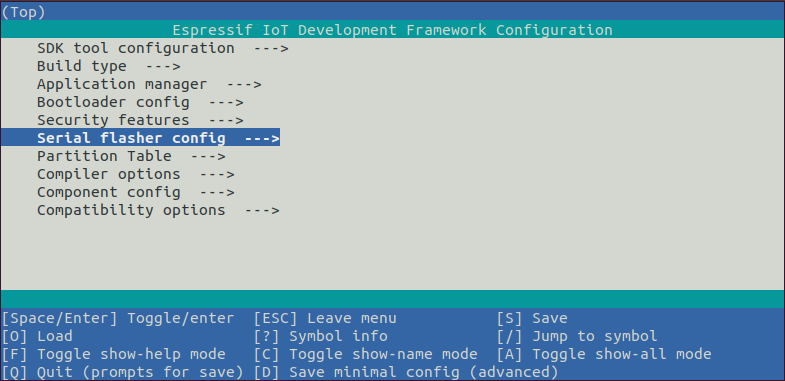
\includegraphics[width=0.9\textwidth]{project-configuration.png}
\caption{配置界面示意图}
\end{figure}

可以通过此菜单设置项目的具体变量,包括 Wi-Fi 网络名称、密码和处理器速度等。\Colorbox{lightgrey}{\lstinline{hello_world}} 示例项目会以默认配置运行,因此在这一项目中,可以跳过使用 menuconfig 进行项目配置这一步骤。

\section{编译工程}

请使用以下命令,编译烧录工程:

\begin{mycode}{编译工程的命令}
idf.py build
\end{mycode}

运行以上命令可以编译应用程序和所有 ESP-IDF 组件,接着生成引导加载程序、分区表和应用程序二进制文件。

\begin{mycode}{运行示意图}
$ idf.py build
Running cmake in directory /path/to/hello_world/build
Executing "cmake -G Ninja --warn-uninitialized /path/to/hello_world"...
Warn about uninitialized values.
-- Found Git: /usr/bin/git (found version "2.17.0")
-- Building empty aws_iot component due to configuration
-- Component names: ...
-- Component paths: ...

... (more lines of build system output)

[527/527] Generating hello_world.bin
esptool.py v2.3.1

Project build complete. To flash, run this command:
../../../components/esptool_py/esptool/esptool.py -p (PORT) -b 921600 write_flash --flash_mode dio --flash_size detect --flash_freq 40m 0x10000 build/hello_world.bin  build 0x1000 build/bootloader/bootloader.bin 0x8000 build/partition_table/partition-table.bin
or run 'idf.py -p PORT flash'
\end{mycode}

如果一切正常,编译完成后将生成 \Colorbox{lightgrey}{\lstinline{.bin}} 文件。

\section{烧录到设备}

请运行以下命令,将刚刚生成的二进制文件烧录至 ESP32 开发板:

\begin{mycode}{编译加烧录}
idf.py flash
\end{mycode}

\begin{marker}
勾选 flash 选项将自动编译并烧录工程,因此无需再运行 \Colorbox{lightgrey}{\lstinline{idf.py build}}。
\end{marker}

\section{常规操作}

在烧录过程中,会看到类似如下的输出日志:

\begin{mycode}{输出日志}
...
esptool.py --chip esp32 -p /dev/ttyUSB0 -b 460800 --before=default_reset --after=hard_reset write_flash --flash_mode dio --flash_freq 40m --flash_size 2MB 0x8000 partition_table/partition-table.bin 0x1000 bootloader/bootloader.bin 0x10000 hello_world.bin
esptool.py v3.0-dev
Serial port /dev/ttyUSB0
Connecting........_
Chip is ESP32D0WDQ6 (revision 0)
Features: WiFi, BT, Dual Core, Coding Scheme None
Crystal is 40MHz
MAC: 24:0a:c4:05:b9:14
Uploading stub...
Running stub...
Stub running...
Changing baud rate to 460800
Changed.
Configuring flash size...
Compressed 3072 bytes to 103...
Writing at 0x00008000... (100 %)
Wrote 3072 bytes (103 compressed) at 0x00008000 in 0.0 seconds (effective 5962.8 kbit/s)...
Hash of data verified.
Compressed 26096 bytes to 15408...
Writing at 0x00001000... (100 %)
Wrote 26096 bytes (15408 compressed) at 0x00001000 in 0.4 seconds (effective 546.7 kbit/s)...
Hash of data verified.
Compressed 147104 bytes to 77364...
Writing at 0x00010000... (20 %)
Writing at 0x00014000... (40 %)
Writing at 0x00018000... (60 %)
Writing at 0x0001c000... (80 %)
Writing at 0x00020000... (100 %)
Wrote 147104 bytes (77364 compressed) at 0x00010000 in 1.9 seconds (effective 615.5 kbit/s)...
Hash of data verified.

Leaving...
Hard resetting via RTS pin...
Done
\end{mycode}

如果一切顺利,烧录完成后,开发板将会复位,应用程序 \Colorbox{lightgrey}{\lstinline{hello_world}} 开始运行。

\section{监视输出}

使用 \textcolor{red}{串口助手} 监视输出和调试。

\begin{marker}
当要进行烧写时,请关闭串口助手!
\end{marker}

\chapter{GPIO操作}

\begin{mycode}{基本配置}
gpio_config_t io_conf;
// 禁用中断
io_conf.intr_type = GPIO_INTR_DISABLE;
// 设置GPIO为输出模式
io_conf.mode = GPIO_MODE_OUTPUT;
// 设置GPIO PIN引脚为 GPIO1 和 GPIO2
io_conf.pin_bit_mask = ((1ULL << GPIO_NUM_1) | (1ULL << GPIO_NUM_2));
// 禁用下拉模式
io_conf.pull_down_en = 0;
// 开启上拉模式
io_conf.pull_up_en = 1;
// 使用以上配置来配置GPIO
gpio_config(&io_conf);
\end{mycode}

\begin{mycode}{配置中断}
// 上升沿触发中断
io_conf.intr_type = GPIO_INTR_POSEDGE;
// 设置为输入模式
io_conf.mode = GPIO_MODE_INPUT;
// 配置引脚
io_conf.pin_bit_mask = (1ULL << GPIO_NUM_0);
gpio_config(&io_conf);
\end{mycode}

\begin{mycode}{操作GPIO引脚}
// 将GPIO口设置为输入模式
gpio_set_direction(GPIO_NUM_2, GPIO_MODE_INPUT);
// 设置输出模式
gpio_set_direction(GPIO_NUM_2, GPIO_MODE_OUTPUT);
// 输出高低电平
gpio_set_level(GPIO_NUM_1, 1);
gpio_set_level(GPIO_NUM_1, 0);
// 获取GPIO的电平
gpio_get_level(GPIO_NUM_2);
\end{mycode}

有了这些API,我们可以实现 $I^2C$ 协议了。然后就可以实现按键功能了。键盘电路图如下:

\begin{figure}[!htb]
\centering
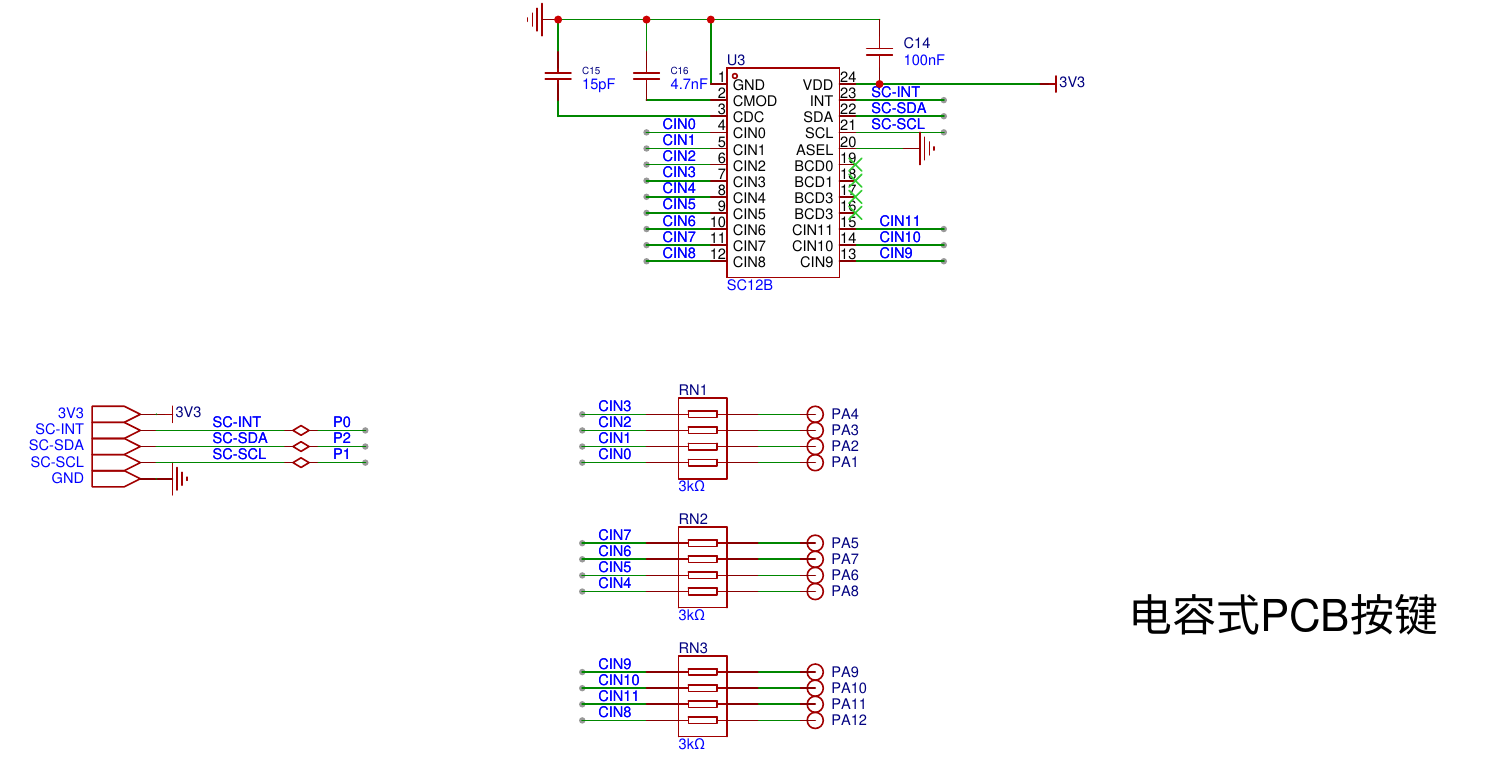
\includegraphics[width=0.9\textwidth]{keyboard.png}
\caption{键盘电路图}
\end{figure}

为了方便操作,我们先来定义一组宏定义以及声明头文件。

先在 main 文件夹中创建 drivers 文件夹,然后创建文件 \Colorbox{lightgrey}{\lstinline{keyboard_driver.h}} 。文件内容如下:

\begin{mycode}{keyboard\_driver.h}
#ifndef __KEYBOARD_DRIVER_H_
#define __KEYBOARD_DRIVER_H_

#include <inttypes.h>
#include "freertos/FreeRTOS.h"
#include "freertos/task.h"
#include "driver/gpio.h"

#define SC12B_SCL GPIO_NUM_1
#define SC12B_SDA GPIO_NUM_2
#define SC12B_INT GPIO_NUM_0

#define I2C_SDA_IN gpio_set_direction(SC12B_SDA, GPIO_MODE_INPUT)
#define I2C_SDA_OUT gpio_set_direction(SC12B_SDA, GPIO_MODE_OUTPUT)

#define I2C_SCL_H gpio_set_level(SC12B_SCL, 1)
#define I2C_SCL_L gpio_set_level(SC12B_SCL, 0)

#define I2C_SDA_H gpio_set_level(SC12B_SDA, 1)
#define I2C_SDA_L gpio_set_level(SC12B_SDA, 0)

#define I2C_READ_SDA gpio_get_level(SC12B_SDA)

void Delay_ms(uint8_t time);
void I2C_Start(void);
void I2C_Stop(void);
void I2C_Ack(uint8_t x);
uint8_t I2C_Wait_Ack(void);
void I2C_Send_Byte(uint8_t d);
uint8_t I2C_Read_Byte(uint8_t ack);
uint8_t SendByteAndGetNACK(uint8_t data);
uint8_t I2C_Read_Key(void);
uint8_t KEYBOARD_read_key(void);
void KEYBORAD_init(void);

#endif
\end{mycode}

然后实现对应的 \Colorbox{lightgrey}{\lstinline{.c}} 文件。

在 drivers 文件夹中创建 \Colorbox{lightgrey}{\lstinline{keyboard_driver.c}} 文件。内容如下:

\begin{mycode}{keyboard\_driver.c}
#include "keyboard_driver.h"

/// 延时函数,使用 FreeRTOS 的 API 进行包装
void Delay_ms(uint8_t time)
{
    vTaskDelay(time / portTICK_PERIOD_MS);
}

/// 产生起始信号
void I2C_Start(void)
{
    I2C_SDA_OUT; // sda线输出
    I2C_SDA_H;
    I2C_SCL_H;
    Delay_ms(1);
    I2C_SDA_L; // START:when CLK is high,DATA change form high to low
    Delay_ms(1);
    I2C_SCL_L; // 钳住I2C总线,准备发送或接收数据
    Delay_ms(1);
}

/// 产生停止信号
void I2C_Stop(void)
{
    I2C_SCL_L;
    I2C_SDA_OUT; // sda线输出
    I2C_SDA_L;   // STOP:when CLK is high DATA change form low to high
    Delay_ms(1);
    I2C_SCL_H;
    Delay_ms(1);
    I2C_SDA_H; // 发送I2C总线结束信号
}

/// 下发应答
void I2C_Ack(uint8_t x)
{
    I2C_SCL_L;
    I2C_SDA_OUT;
    if (x)
    {
        I2C_SDA_H;
    }
    else
    {
        I2C_SDA_L;
    }
    Delay_ms(1);
    I2C_SCL_H;
    Delay_ms(1);
    I2C_SCL_L;
}

/// 等待应答信号到来,成功返回 0 。
uint8_t I2C_Wait_Ack(void)
{
    uint8_t ucErrTime = 0;
    I2C_SCL_L;
    I2C_SDA_IN; // SDA设置为输入
    Delay_ms(1);
    I2C_SCL_H;
    Delay_ms(1);
    while (I2C_READ_SDA)
    {
        if (ucErrTime++ > 250)
        {
            // I2C_Stop();
            // printf("接受应答失败\n");
            return 1;
        }
    }
    I2C_SCL_L;
    // printf("接受应答成功\n");
    return 0;
}

/// 发送一个字节
void I2C_Send_Byte(uint8_t d)
{
    uint8_t t = 0;
    I2C_SDA_OUT;
    while (8 > t++)
    {
        I2C_SCL_L;
        Delay_ms(1);
        if (d & 0x80)
        {
            I2C_SDA_H;
        }
        else
        {
            I2C_SDA_L;
        }
        Delay_ms(1); // 对TEA5767这三个延时都是必须的
        I2C_SCL_H;
        Delay_ms(1);
        d <<= 1;
    }
}

/// 读 1 个字节
uint8_t I2C_Read_Byte(uint8_t ack)
{
    uint8_t i = 0;
    uint8_t receive = 0;
    I2C_SDA_IN; // SDA设置为输入
    for (i = 0; i < 8; i++)
    {
        I2C_SCL_L;
        Delay_ms(1);
        I2C_SCL_H;
        receive <<= 1;
        if (I2C_READ_SDA)
        {
            receive++;
        }
        Delay_ms(1);
    }
    I2C_Ack(ack); // 发送ACK
    return receive;
}

/// 发送数据并返回应答
uint8_t SendByteAndGetNACK(uint8_t data)
{
    I2C_Send_Byte(data);
    return I2C_Wait_Ack();
}

/// SC12B 简易读取按键值函数(默认直接读取)
/// 此函数只有初始化配置默认的情况下,直接调用,
/// 如果在操作前有写入或者其他读取不能调用默认
uint8_t I2C_Read_Key(void)
{
    I2C_Start();
    if (SendByteAndGetNACK((0x40 << 1) | 0x01))
    {
        I2C_Stop();
        return 0;
    }
    uint8_t i = 0;
    uint8_t k = 0;
    I2C_SDA_IN; // SDA设置为输入
    while (8 > i)
    {
        i++;
        I2C_SCL_L;
        Delay_ms(1);
        I2C_SCL_H;
        if (!k && I2C_READ_SDA)
        {
            k = i;
        }
        Delay_ms(1);
    }
    if (k)
    {
        I2C_Ack(1);
        I2C_Stop();
        return k;
    }
    I2C_Ack(0);
    I2C_SDA_IN; // SDA设置为输入
    while (16 > i)
    {
        i++;
        I2C_SCL_L;
        Delay_ms(1);
        I2C_SCL_H;
        if (!k && I2C_READ_SDA)
        {
            k = i;
        }
        Delay_ms(1);
    }
    I2C_Ack(1);
    I2C_Stop();
    return k;
}

uint8_t KEYBOARD_read_key(void)
{
    uint16_t key = I2C_Read_Key();
    if (key == 4)
    {
        return 1;
    }
    else if (key == 3)
    {
        return 2;
    }
    else if (key == 2)
    {
        return 3;
    }
    else if (key == 7)
    {
        return 4;
    }
    else if (key == 6)
    {
        return 5;
    }
    else if (key == 5)
    {
        return 6;
    }
    else if (key == 10)
    {
        return 7;
    }
    else if (key == 9)
    {
        return 8;
    }
    else if (key == 8)
    {
        return 9;
    }
    else if (key == 1)
    {
        return 0;
    }
    else if (key == 12)
    {
        return '#';
    }
    else if (key == 11)
    {
        return 'M';
    }
    return 255;
}

/// GPIO初始化
void KEYBORAD_init(void)
{
    gpio_config_t io_conf;
    // disable interrupt
    io_conf.intr_type = GPIO_INTR_DISABLE;
    // set as output mode
    io_conf.mode = GPIO_MODE_OUTPUT;
    // bit mask of the pins that you want to set,e.g.SDA
    io_conf.pin_bit_mask = ((1ULL << SC12B_SCL) | (1ULL << SC12B_SDA));
    // disable pull-down mode
    io_conf.pull_down_en = 0;
    // disable pull-up mode
    io_conf.pull_up_en = 1;
    // configure GPIO with the given settings
    gpio_config(&io_conf);

    // 中断
    io_conf.intr_type = GPIO_INTR_POSEDGE;
    io_conf.mode = GPIO_MODE_INPUT;
    io_conf.pin_bit_mask = (1ULL << SC12B_INT);
    gpio_config(&io_conf);
}
\end{mycode}

驱动编写好之后,我们可以在主函数中和电容键盘进行通信了。当按下按键,会产生中断,通过处理中断来识别我们的按键。

在 \Colorbox{lightgrey}{\lstinline{smart-lock.c}} 文件中,主函数是:\Colorbox{lightgrey}{\lstinline{app_main}},ESP-IDF 在编译整个项目的时候,会将 \Colorbox{lightgrey}{\lstinline{app_main}} 注册为一个RTOS任务。无需我们自己编写 main 函数。参见文件中的第 \ref{line:sp} 行。

\begin{mycode}{smark-lock.c}
// 全局变量,用来存储来自 GPIO 的中断事件
static QueueHandle_t gpio_evt_queue = NULL;

static void IRAM_ATTR gpio_isr_handler(void *arg)
{
  uint32_t gpio_num = (uint32_t)arg;
  // 将产生中断的GPIO引脚号入队列。
  xQueueSendFromISR(gpio_evt_queue, &gpio_num, NULL);
}

// 轮询中断事件队列,然后挨个处理
static void process_isr(void *arg)
{
  uint32_t io_num;
  for (;;)
  {
    if (xQueueReceive(gpio_evt_queue, &io_num, portMAX_DELAY))
    {
      if (io_num == 0)
      {
        uint8_t key = KEYBOARD_read_key();
        printf("按下的键:%d\r\n", key);
      }
    }
  }
}

static void ISR_QUEUE_Init(void)
{
  // 创建一个队列来处理来自GPIO的中断事件
  gpio_evt_queue = xQueueCreate(10, sizeof(uint32_t));
  // 开启 process_isr 任务。
  // 这个任务的作用是轮训存储中断事件的队列,将队列中的事件
  // 挨个出队列并进行处理。
  xTaskCreate(process_isr, "process_isr", 2048, NULL, 10, NULL);

  gpio_install_isr_service(0);
  // 将 SC12B_INT 引脚产生的中断交由 gpio_isr_handler 处理。
  // 也就是说一旦 SC12B_INT 产生中断,则调用 gpio_isr_handler 函数。
  gio_isr_handler_add(SC12B_INT, gpio_isr_handler, (void *)SC12B_INT);
}

// 主程序
void app_main(void) @\label{line:sp}@
{
  ISR_QUEUE_Init();
}
\end{mycode}

\end{document}